\documentclass[11pt]{article}

\usepackage[utf8]{inputenc}
\usepackage[german]{babel}

\usepackage[a4paper,top=2.5cm,bottom=2.5cm,left=3cm,right=2.5cm]{geometry}

% Set arial font
\usepackage{helvet}
\renewcommand{\familydefault}{\sfdefault}

% Allow for special characters such as < >
\usepackage[T1]{fontenc}
% Modify the figure caption font
\usepackage[font=small,labelfont=bf]{caption}

\usepackage{amsmath}
\usepackage{amsthm}

\usepackage{graphicx}
\usepackage[colorlinks=true, allcolors=blue]{hyperref}

\usepackage{minted}
\graphicspath{{./images/}} 
 

\usepackage{csquotes}
\usepackage[style=numeric,sorting=ynt]{biblatex}
\addbibresource{main.bib}

% Hypthenation rules
\hyphenation{
  zu-sam-men-ge-setzt-er 
  ma-the-ma-tisch-en
  ver-wen-den
  dar-zu-stel-len
  ent-ge-gen-zu-neh-men
  un-ter-such-en
  ato-ma-rer
  zu-ein-an-der
  Ope-ra-tor-rang-fol-ge
  er-for-der-lich
  Re-geln
  Im-ple-men-tie-rung
  ge-ne-rie-ren
}


\newtheorem{defin}{Definition}
\newcommand{\lab}[1]{(Def. \ref{#1})}

\newtheorem{example}{Beispiel}

% Apparently a linespreach of 1.25 is equal to a 1.5 linespacing in word
\linespread{1.25}
% No indent for parapgraphs
\setlength\parindent{0pt}

\title{Computer Algebra Systeme}
\author{Simon Weckler}

\begin{document}

\maketitle
\tableofcontents

\section{Einleitung}

Seit Anbeginn der Mathematik existiert  die Nachfrage nach Rechenhilfsmitteln.
Was 300 vor Christus noch der Abakus war, sind heute Computeralgebrasysteme.
Diese Systeme sind für Studenten, Forschung und Industrie ein unerlässliches Werkzeug
und bilden ein eigenes Marktsegment.\\

Aus der Definition von Computeralgebra von der \citeauthor{CA} \cite{CA}
lässt sich folgende Definition für ein Computeralgebrasystem ableiten:
\begin{defin}
\label{def:cas}
Ein Computeralgebrasystem ist ein Programm, welches Methoden zum Lösen mathematisch
formulierter Probleme durch symbolische Algorithmen bietet. Es beruht auf der exakten
endlichen Darstellung mathematischer Objekte und Strukturen.
Das Rechnen mit beliebig langen Zahlen, Symbolen, Unbestimmten und Polynomen, 
das Faktorisieren von Zahlen und Polynomen, das Differenzieren von Polynomen und 
anderen Funktionen und das exakte Lösen von Differenzialgleichungen 
sind einige konkrete Beispiele für Problemstellungen, die die meisten Computeralgebrasysteme
lösen können.

Damit ein Computeralgebrasystem nützlich ist, sollte es folgende Eigenschaften haben:
\begin{enumerate}
  \item Eine Benutzeroberfläche, über die der Benutzer mathematische Ausdrücke eingeben kann.
  \item Einen Vereinfachungsalgorithmus welcher mathematiche Ausdrücke vereinfachen kann.
  \item Eine große Menge an mathematischen Algorithmen und Funktionen. Dazu gehören zum Beispiel
        Algorithmen zur Bestimmung der Ableitung eines Terms.
  \item Eine eigene Programmierumgebung, insbesondere eine eigene Programmiersprache.
\end{enumerate}

\end{defin}

In dieser Arbeit soll nachvollzogen werden, wie Computeralgebrasysteme mit den Texteingaben von Benutzern 
umgehen und diese intern darstellen. Außerdem soll die Funktionsweise eines Computeralgebrasystem 
anhand des Algorithmus der automatischen Vereinfachung dargestellt werden.
Um dies zu erreichen, wurde ein eigenes, simples Computeralgebrasystem implementiert,
welches die Texteingabe des Benutzers einlesen, auswerten und vereinfachen kann. 
Zudem wird es zur Visualisierung von Beispielen verwendet und dient als Möglichkeit, 
selbst Eingaben auszuprobieren. 

Im Zusammenhang dieser Arbeit wurde die Website \url{https://cas.dotenv.de} erstellt.
In der Website wurden die Algorithmen, welcher in dieser Arbeit vorgestellt werden implementiert
und können visuell nachvollzogen werden.

\section{Benutzereingaben}
Die einfachste Form, einen mathematischen Ausdruck auf einem Computer einzugeben, 
ist unter der Verwendung der Symbole, welche einem auf der Tastatur schon zur Verfügung stehen. 
Dabei gelten folgende Beziehungen zwischen den Zeichen und ihrer mathematischen Bedeutung:
\begin{table}[h]
\begin{tabular}{|l|l|}
\hline
  Zeichen               & Bedeutung         \\ \hline \hline
  0 - 9                 & Ziffer            \\ \hline
  +                     & Addition          \\ \hline
  -                     & Subtraktion        \\ \hline
  /                     & Division          \\ \hline
  *                     & Multiplikation    \\ \hline
  \textasciicircum      & Potenz            \\ \hline
  a - z                 & Symbol (Variable) \\ \hline
\end{tabular}
\end{table}

Es ist mit nur diesen Zeichen möglich, eine Großzahl von mathematischen Termen darzustellen 
und ist deswegen ein simpler, aber effektiver Weg, um Benutzereingaben entgegenzunehmen.

\subsection{Darstellung im Programm}
\subsubsection{Darstellung als String}

Der Benutzer kann einen mathematischen Ausdruck also in Form eines Strings eingeben. 
Den String auch als Datenstruktur zur Darstellung des Ausdrucks im Programm zu 
verwenden hat allerdings Nachteile. 
Um zu beurteilen, ob eine Darstellung als String für einen Computer passend ist oder nicht, 
muss zuerst definiert werden, welche Informationen das Programm benötigt,
um mit dem Term arbeiten zu können.

\begin{defin}
  Um mit einem mathematischen Term arbeiten zu können muss ein Programm die Bedeutung
  der einzelnen Zeichen sowie die Operatorrangfolge \lab{def:operatorrangfolge} kennen.
\label{def:programm_infos}
\end{defin}

\begin{defin}
Unter der \textbf{Operatorrangfolge} oder \textbf{Operatorpräzedenz} ist die Ordnung zu verstehen, 
in welcher die Operatoren eines Ausdrucks auszuwerten sind.
In dem Term $3+4*5$ hat der Operator $+$ die geringste Priorität und der Operator $*$ die höchste. 
Folglich muss $4*5$ vor $3+4$ ausgerechnet werden. 
\label{def:operatorrangfolge}
\end{defin}

Ein String bietet sich folglich nicht als Datenstruktur für einen mathematischen Ausdruck 
an, da weder die Operatorpräzedenz noch die Bedeutung der Zeichen klar ersichtlich ist.
Für ein Programm existiert schließlich per se kein Unterschied zwischen dem Zeichen $3$ und $+$, 
da beide denselben Datentyp (\textit{char}) haben.

\subsubsection{Darstellung als Baum}

Ideal wäre also eine Datenstruktur, welche sowohl die Bedeutung der Zeichen als auch die Operatorrangfolge speichert,
sodass diese nicht neu berechnet werden müssen. \newline
Laut \citeauthor{CAS_EA} \cite[81]{CAS_EA} entweder als atomarer 
oder zusammengesetzter Ausdruck klassifiziert werden kann.

\begin{defin}
Ein \textbf{atomarer Ausdruck} ist jeder Ausdruck, der kein Operator ist, also ganze Zahlen und Symbole. 
Atomare Ausdrücke können nicht weiter vereinfacht werden.
\label{def:atomarer_ausdruck}
\end{defin}

\begin{defin}
Jeder \textbf{zusammengesetzte Ausdruck} besteht aus einem Operator und einem oder mehreren Operanden. 
Zu diesen Ausdrücken zählen Summen, Produkte, Differenzen, Divisionen und Potenzen
\label{def:zusammengesetzter_ausdruck}
\end{defin}

Man kann nun atomare und zusammengesetzte Ausdrücke und ihre Beziehungen zueinander in einem Baum darstellen.
Dabei gelten folgende Regeln:

\begin{defin}
In einem \textbf{Baum mathematischer Ausdrücke} ist jeder Elternknoten ein zusammengesetzter Ausdruck. Die Kinder
eines Elternknotens sind seine Operanden, welche Zusammengesetze \lab{def:zusammengesetzter_ausdruck} oder atomare 
\lab{def:atomarer_ausdruck} Ausdrücke sein können. Alle Blätter des Baumes sind atomare Ausdrücke. \lab{def:atomarer_ausdruck}
\label{def:baum}
\end{defin}

\begin{figure}[h]
  \centering
  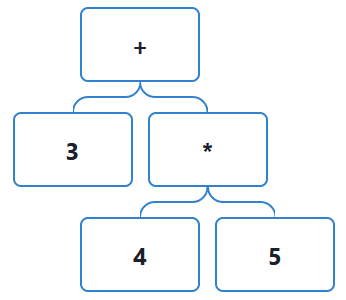
\includegraphics[scale=0.5]{trees/beispiel_1_baum.png}
  \caption{Der Baum für den Term $3+4*5$.}
\end{figure}

\begin{example}
   An dem Baum für den Term $3+4*5$ kann man erkennen, dass die Operatorrangfolge \lab{def:operatorrangfolge}
   in der Datenstruktur abgebildet wird. Da der Ausdruck $4*5$ ein Kind des Operators $+$ ist, muss dieser zuerst 
   ausgewertet werden. In einem Baum mathematischer Ausdrücke \lab{def:baum} ist die Wurzel folglich immer
   der Operator mit der geringsten Priorität.
   Wie man außerdem erkennen kann, sind alle Blätter des Baumes ganze Zahlen, also atomare Ausdrücke \lab{def:atomarer_ausdruck}.
\end{example}

Von welchem Datentyp die Blätter und Knoten sind, ist ganz von der eigenen Implementierung abhängig.
In diesem Computer Algebra System können folgende Ausdrücke Teil des Baumes sein:

\begin{figure}[h]
  \centering
  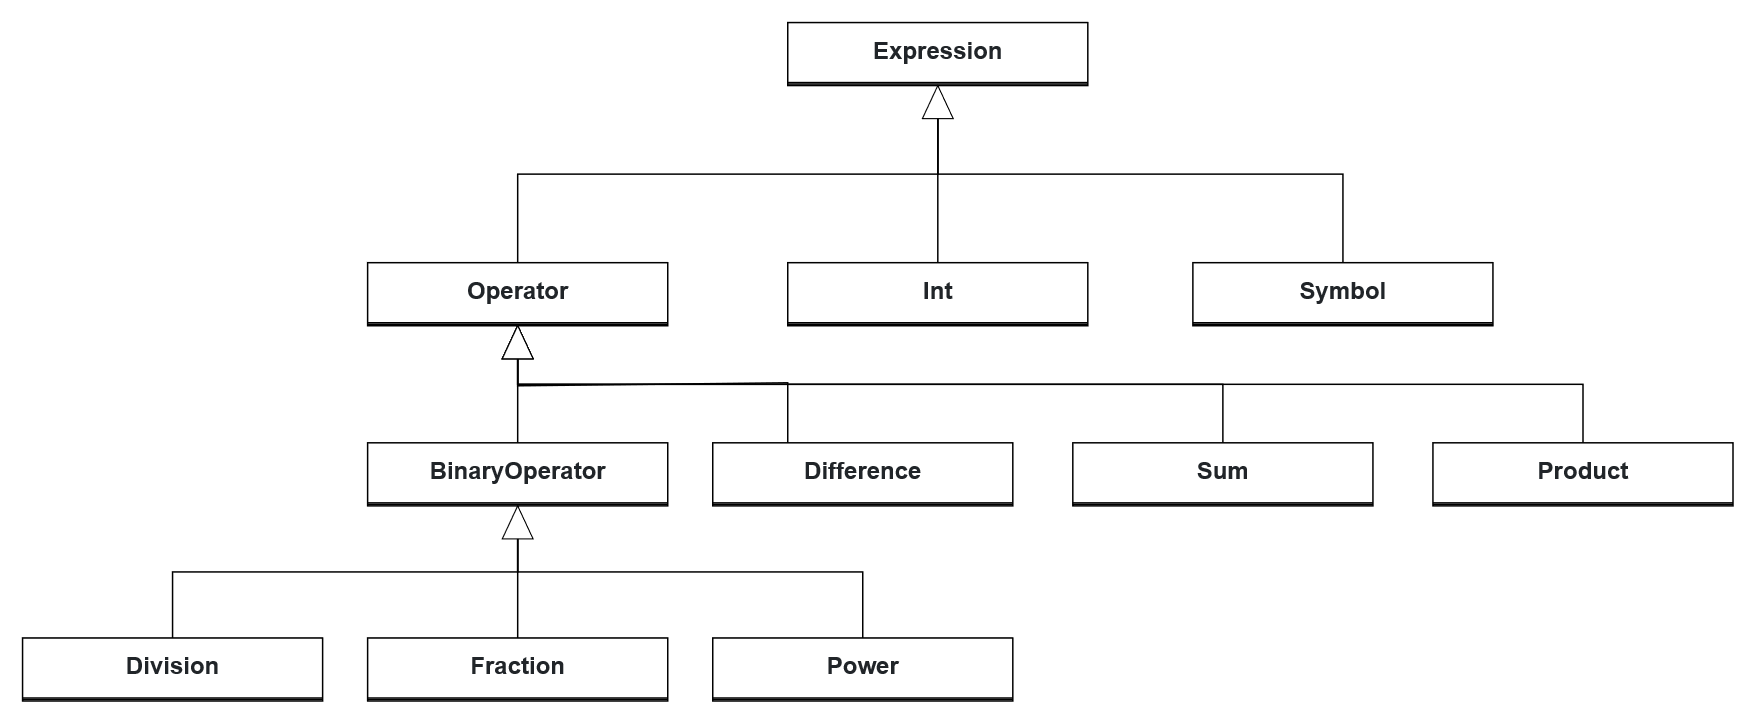
\includegraphics[scale=0.25]{UML_Ausdruecke.png}
  \caption{UML Diagramm aller Ausdrücke.}
\end{figure}

Hier wurden die Operatoren in Binäre und Nicht-Binäre Operatoren unterteilt.
\begin{defin}
  \textbf{Binäre Operatoren} sind Operatoren, welche immer zwei Operanden haben müssen.
\end{defin} 
\begin{defin}
  \textbf{Nicht-Binäre Operatoren} sind Operatoren, deren Operanden-zahl aufgrund des
  Assoziativgesetzes zwischen 1 und N variieren kann.
\end{defin}

Wie einem vielleicht auffällt, ist auch der Bruch ein Operator. 
Das ist darin begründet, dass ein Bruch genau genommen auch eine Operation (Division) ist, 
allerdings eine, die nicht zu einer ganzen Zahl vereinfacht werden kann. 
Im Baum wird ein Bruch also wie folgt dargestellt:

\begin{figure}[h]
  \centering
  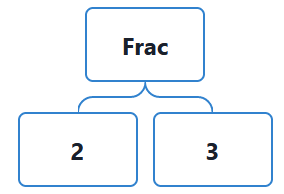
\includegraphics[scale=0.5]{trees/beispiel_baum_frac.png}
  \caption{Ein Bruch im Baum mathematischer Ausdrücke.}
\end{figure}

\subsection{Parsen}
In einem Computeralgebrasystem wird ein Term also in Form eines Baumes dargestellt. 
Für den Benutzer wäre es allerdings weder intuitiv noch einfach, einen Term als Baum anzugeben. 
Die Eingabe als String sollte also beibehalten werden. 
Folglich ist es erforderlich, die Zeichenkette nach Eingabe in einen Baum umzuwandeln.
Um die Struktur der Eingaben zu kennen ist es notwendig diese zu definieren. Hier wurde
die Definition \citeauthor{CAS_EA}s \cite[86 - 87]{CAS_EA} leicht abgeändert. Insbesondere
wurde die Anzahl möglicher Operatoren reduziert.

\begin{defin}
  \label{def:konventionelle_struktur}
  Die \textbf{konventionelle Struktur} eines Ausdrucks entspricht der Struktur vor der automatischen Vereinfachung. 
  Diese Struktur ist auch die, die in der Mathematik verwendet wird. Hier gilt:

  \begin{enumerate}
    \item die Operatoren $+$ und $-$ haben entweder 1 oder 2 Operanten.
    \item die Operatoren $*$, $/$, und \textrm{\textasciicircum} haben immer 2 Operanten.
    \item die Operanden der Operatoren  sind Algebraische Ausdrücke.
  \end{enumerate}

  Jeder Ausdruck kann immer einem Klammerlevel zugeordnet werden. 
  Standardmäßig ist das Klammerlevel 0. Befindet sich ein Ausdruck in runden Klammern, 
  so erhöht sich sein Klammerlevel um 1. Der Ausdruck mit dem höheren Klammerlevel hat immer die höhere Priorität 
  gegenüber einem Ausdruck mit niedrigerem Klammerlevel.
  Es gelten folgende Regeln für die Operatorrangfolge \lab{def:operatorrangfolge} bei gleichem Klammerlevel:

  \begin{center}
    Höchste Priorität \\
    \textrm{\textasciicircum} \\
    \textrm{* /} \\
    \textrm{+ -} \\
    Niedrigste Priorität
  \end{center}

  Falls 2 Operatoren dieselbe Priorität haben (z. B. + und -) hat 
  der rechte Operator die höhere Priorität.
  Die einzige Ausnahme ist die Potenz, bei welcher der linke Operator
  die höhere Priorität hat.
\end{defin}

Um aus diesen Regeln einen Algorithmus zu bauen, ist es hilfreich, 
eine Grammatik für einen mathematischen Ausdruck unter Beachtung der eben definierten Regeln 
in Form einer Backus-Naur-Form zu definieren. 

\begin{defin}
  Eine \textbf{Backus-Naur-Form} (BNF) ist nach der Definition von \citeauthor{A_COMP} \cite{A_COMP}
  eine Notationsform, um die Grammatik von Sprachen zu definieren. 
  Der Syntax einer Backus-Naur-Form ist sehr einfach zu verstehen, da es nur 3 Symbole gibt.  

  \begin{table}[h]
  \begin{tabular}{|l|l|}
  \hline
    Zeichen     & Bedeutung               \\ \hline
    ::=         & Ist definiert als       \\ \hline
    |           & Oder                    \\ \hline
    <X>         & Name einer Kategorie X  \\ \hline
  \end{tabular}
  \end{table}
\end{defin}

\begin{minted}{bnf}
<Addition>    ::=    <Ziffer> + <Ziffer>
<Ziffer>      ::=    0 | 1 | 2 | 3 | 4 | 5 | 6 | 7 | 8 | 9 
\end{minted}
Diese Backus-Naur-Form kann gelesen werden als: 
Eine Addition besteht aus 2 Ziffern, 
welche durch ein Plus Symbol getrennt sind. 
Eine Ziffer ist eine Zahl von 0 bis 9. 
Wie einem vielleicht auffällt, erlaubt diese Definition nur 
die Addition von 2 Ziffern. Der String $32+2$ würde also nicht 
dieser Definition einer Addition entsprechen. \newline \\
Um einen String nun in einen Baum auf Basis einer Backus-Naur-Form umzuwandeln, 
lässt sich folgender Algorithmus formulieren

\begin{defin}
  Algorithmus zum Parsen eines BNF Baums
  \begin{enumerate}
    \item Überprüfe, ob der gegebene String der 1. Option der jeweiligen Definition entspricht.
    \item Ist die Definition abhängig von einer weiteren Definition, so überprüfe ob der String oder Teilstring auch der Kinddefinition entspricht.
    \item Entspricht der String der Definition, so erweitere den Baum mit dem passenden Knoten / Blatt.
    \item Ist das nicht der Fall, so probiere die nächste Option. Gibt es keine weitere Option mehr, so muss es sich um einen invaliden String handeln.
  \end{enumerate}
\end{defin}

Wenden wir diesen Algorithmus an, 
entsteht ein Baum für den gegebenen Term.
Die vorher definierte Backus-Naur-Form würde 
zum Beispiel für den Input $2+3$ folgenden Baum generieren.

\begin{figure}[h]
  \centering
  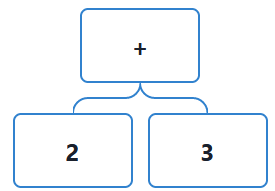
\includegraphics[scale=0.5]{trees/beispiel_bnf_1.png}
  \caption{Parse Tree für den Input $2+3$.}
\end{figure}

Ziel ist es nun, eine Backus-Naur-Form für einen mathematischen Ausdruck 
zu definieren, welche alle Aspekte der Definition 
eines mathematischen Ausdrucks in der konventionellen Struktur 
\lab{def:konventionelle_struktur} berücksichtigt. Dabei dient die
Definition einer Backus-Naur-Form für mathematische Ausdrücke von \citeauthor{BNF_PT}
\cite{BNF_PT} als Vorlage.

\begin{minted}{bnf}
<exp>       ::= <exp> + <exp> | <exp> * <exp> | <exp> - <exp> | 
                <exp> / <exp> | <exp> ^ <exp> | <int> | <symbol>
<int>       ::= <digit> <int> | <digit>
<digit>     ::= 0 | 1 | 2 | 3 | 4 | 5 | 6 | 7 | 8 | 9 | 10
<symbol>    ::= a | b | c | d | e | f | g | h | i | j | k | l | m | n | 
                o | p | q | s | t | u | v | w | x | y | z
\end{minted}

Diese Grammatik ist in der Lage, eine große Anzahl von Ausdrücken zu repräsentieren. 
So zum Beispiel auch $6+3*4$. Bei genauerer Betrachtung fällt einem jedoch auf, 
dass diese Grammatik die Operatorpräzedenz \lab{def:operatorrangfolge} 
nicht berücksichtigt. 
Es gibt für den Term $6+3*4$ zwei verschiedene Bäume, 
die mit der Grammatik übereinstimmen. 
Allerdings ist nur der 1. Baum korrekt. 

\begin{figure}[h]
\begin{minipage}{.5\textwidth}
  \centering
  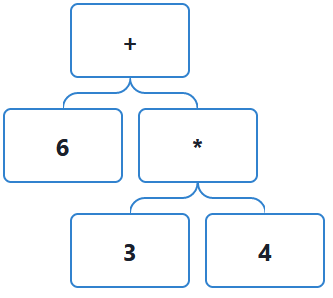
\includegraphics[scale=0.5]{trees/beispiel_bnf_2_1.png}
  \caption{1. Möglicher Baum für $6+3*4$.}
\end{minipage}
\begin{minipage}{.5\textwidth}
  \centering
  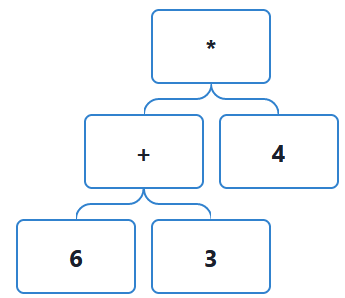
\includegraphics[scale=0.5]{trees/beispiel_bnf_2_2.png}
  \caption{2. Möglicher Baum für $6+3*4$.}
\end{minipage}
\end{figure}

Dieses Problem kann dadurch gelöst werden, dass man eine Multiplikation als 
Operand einer Addition erlaubt, aber Addition nicht als Operand der Multiplikation 
zulässt. Diese Änderung resultiert in folgendem BNF:

\begin{minted}{bnf}
<exp>     ::= <exp> + <exp> | <exp> - <exp> | 
<term>    ::= <term> * <term> | <term> / <term> | <factor>
<power>   ::= <power> ^ <power>
<factor>  ::= <int> | <symbol 
<int>     ::= <digit> <int> | <digit>
<digit>   ::= 0 | 1 | 2 | 3 | 4 | 5 | 6 | 7 | 8 | 9 | 10
<symbol>  ::= a | b | c | d | e | f | g | h | i | j | k | l | m | n | 
              o | p | q | s | t | u | v | w | x | y | z
\end{minted}

Für den Term $6+3*4$ gibt es nur noch einen möglichen Baum,
allerdings gibt es noch ein weiteres Problem. 
Bei der Subtraktion von mehreren Zahlen, 
zum Beispiel $4-5-2$ gibt es wieder zwei mögliche Bäume 
mit zwei verschiedenen Ergebnissen. 

\begin{figure}[h]
\begin{minipage}{.5\textwidth}
  \centering
  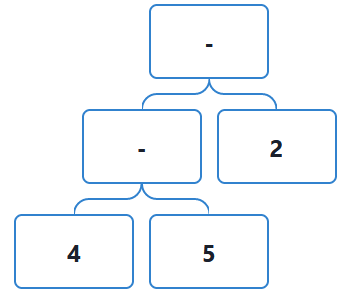
\includegraphics[scale=0.5]{trees/beispiel_bnf_3_1.png}
  \caption{1. Möglicher Baum für $4-5-2$.}
\end{minipage}
\begin{minipage}{.5\textwidth}
  \centering
  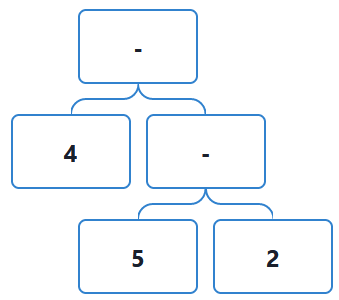
\includegraphics[scale=0.5]{trees/beispiel_bnf_3_2.png}
  \caption{2. Möglicher Baum für $4-5-2$.}
\end{minipage}
\end{figure}

Das Problem entsteht dadurch, dass sowohl die linke als auch 
die rechte Seite der Differenz weitere Differenzen enthalten können. 
Das darf also nur noch auf der linken Seite erlaubt sein. 
Die einzige Ausnahme ist die Potenz, da sie ein rechts assoziativer Operator ist. 
Was außerdem noch fehlt, sind unäre Summen und Differenzen, 
sowie die Möglichkeit, mit Klammern die Operatorrangfolge zu manipulieren. 
Mit allen diesen Änderungen sieht die Backus-Naur-Form nun folgendermaßen aus:

\begin{minted}{bnf}
<exp>     ::= + <term> | <exp> + <term> | - <term> | <exp> - <term> | <term> 
<term>    ::= <term> * <power> | <term> / <power> | <power>
<power>   ::= <factor> ^ <power> | <factor>
<factor>  ::= ( <exp> ) | <int> | <symbol> 
<int>     ::= <digit> <int> | <digit>
<digit>   ::= 0 | 1 | 2 | 3 | 4 | 5 | 6 | 7 | 8 | 9 | 10
<symbol>  ::= a | b | c | d | e | f | g | h | i | j | k | l | m | n | 
              o | p | q | s | t | u | v | w | x | y | z
\end{minted}

Der Algorithmus, der auf dieser Backus-Naur-Form basiert und zum Parsen eines Strings in einen
Baum mathematischer Ausdrücke \lab{def:baum} dient kann im Source Code unter dem Pfad /server/cas/parse.ts 
oder online über \url{https://github.com/Flosi23/cas/blob/main/server/cas/parse.ts} eingesehen werden. \newline
Außerdem bietet sich die Möglichkeit das Verhalten des Algorithmus auf der Website  \url{https://cas.dotenv.de}
direkt selbst auszuprobieren. Dafür muss ein mathematischer Ausdruck welcher der konventionellen Struktur 
entspricht \lab{def:konventionelle_struktur}
(Dabei sollte vor allem beachtet werden, dass zum Beispiel der Term $3x$ als $3*x$ geschrieben werden muss)
in das Eingabefeld eingeben und der Knopf \glqq Calculate\grqq{}  gedrückt werden. 
Der vom Algorithmus generierte Baum kann dann unter dem Reiter \glqq Expression Tree\grqq{} eingesehen werden.

\section{Automatische Vereinfachung}

Jedes Computeralgebrasystem wendet mathematische Regeln an, um einen Ausdruck zu vereinfachen. 
Diesen Prozess nennt man automatische Vereinfachung. 
Jeder Ausdruck wird automatisch vereinfacht, bevor andere Operationen angewendet werden. 
Motivation hinter der automatischen Vereinfachung ist es, den Term in eine einheitliche und simplere Form zu bringen, 
damit man ihn mit anderen Termen vergleichen und damit rechnen kann. 

\begin{example}
Nimmt man den Term $3+x+y$ so gibt es aufgrund des Kommutativgesetzes 6 verschiedene Möglichkeiten diesen
niederzuschreiben ohne, dass sich sein Ergebnis verändert
\begin{enumerate}
  \item $3+x+y$
  \item $3+y+x$
  \item $y+3+x$
  \item $y+x+3$
  \item $x+y+3$
  \item $x+3+y$
\end{enumerate}
\end{example}

Obwohl alle 6 Terme äquivalent sind, sind sie syntaktisch nicht gleich und würden aufgrund dessen von einem Computeralgebrasystem
vor der automatischen Vereinfachung nicht als gleich angesehen werden. Ohne eine Vereinheitlichung könnten die Terme also nicht 
verglichen werden.
Wieso das problematisch ist, lässt sich an einem einfachen Beispiel zeigen.

\begin{example}
  Nehme man den Term $6xy+8yx$. Für einem Menschen ist klar ersichtlich, dass man diesen zu $14xy$ vereinfachen kann.
  Ein Computeralgebrasystem könnte diese Vereinfachung aber nicht vornehmen, da es die Terme $xy$ und $yx$ nicht als gleich
  ansehen und folglich nicht addieren würde. 
\end{example}

Neben der Sortierung ist ein weiterer wichtiger Schritt Operatoren wie Division und Differenz durch andere Operatoren
zu ersetzen, um die Anzahl möglicher Operatoren zu reduzieren und den Baum mathematischer Ausdrücke so zu simplifizieren. \newline
Zuletzt sollen auch alle Zahlenwerte so weit zusammengerechnet werden wie möglich und mathematische Gesetze 
(wie etwa das Distributivgesetz) angewendet werden, um den Term zu vereinfachen.

\begin{defin}
  Basierend auf der Definition \citeauthor{CAS_EA}s \cite[90 92]{CAS_EA} gilt ein Term als
  \textbf{vollständig vereinfacht}, wenn die folgenden Bedingungen erfüllt sind:
  \begin{enumerate}
    \item $+$ ist ein Operator mit mindestens zwei Operanden (aufgrund des Assoziativgesetzes ist es möglich, 
          dass Plus n viele Operanden haben kann) von denen maximal 1 Operand eine Zahl oder ein Bruch sein darf 
          (andernfalls könnte man den Ausdruck noch weiter zusammenfassen).
    \item $*$ ist ein Operator mit mindestens zwei Operanden, von denen keiner ein Produkt sein darf. 
          Auch eine Summe darf kein Operand einer Multiplikation sein, da diese immer mithilfe des Distributivgesetzes
          vereinfacht werden kann.
          Außerdem darf nur maximal ein Operand eine Zahl oder ein Bruch sein. 
    \item Zahlen müssen in Summen und Produkten immer der 1. Operand sein.
    \item Der Operator $-$ darf nicht vorkommen, da er immer als Produkt mit -1 dargestellt werden kann.
    \item Auch der Operator $/$ darf nicht vorkommen, da man einen Quotienten immer als Produkt oder numerischen Bruch darstellen kann.
    \item Ein Quotient, der einen Bruch bei dem sowohl Zähler, und Nenner nicht Null und natürliche Zahlen sind aufweist, 
          muss als Bruch dargestellt werden. Außerdem muss der Nenner größer als eins und der größte gemeinsame Teiler eins sein.
    \item Bei einer Potenz $v^n$ muss $n$ eine natürliche Zahl sein. Außerdem darf $v$ keine eine Zahl, Bruch, Potenz oder ein Produkt sein
  \end{enumerate}
\end{defin}

\subsection{Transformationen}

Folgende Transformationen \citeauthor{CAS_MM}s \cite[64 - 79]{CAS_MM}
stellen die Grundlage eines jeden Algorithmus der automatischen Vereinfachung dar und können,
wenn richtig angewandt einen Term vollständig vereinfachen.

\subsubsection{Distributive Transformation}

\begin{defin}
  \label{def:distributive_transformation}
  Bei der \textbf{distributiven Transformation} werden in Summen 
  gleiche Terme mit konstanten Koeffizienten basierend auf dem Distributivgesetz vereinfacht, 
  indem ihre Koeffizienten miteinander addiert werden. 
  Ist einer der Operanden einer Multiplikation eine Summe so werden die anderen Operanden
  der Multiplikation mit den Operanden der Summe multipliziert.
\end{defin}

\begin{example}
  Anwendung der distributiven Transformation bei einer Summe: \newline
  $2x + y + \frac{3}{2}x = \frac{7}{2}x + y$
\end{example}

\begin{example}
  Anwendung der distributiven Transformation bei einer Multiplikation: \newline
  $6 * x * (3 + y) = 6 * (3x + xy) = 18x + 6xy$
\end{example}

\subsubsection{Assoziative Transformation}

\begin{defin}
  \label{def:assoziative_transformation}
  Existiert ein Term $U$, der eine Summe bzw. ein Produkt ist, und einer der Operanten $S$ ist auch eine Summe 
  bzw. ein Produkt, so werden die Operatoren von $S$ zu $U$ addiert. 
  Diese Transformation wird immer vor der Distributiven Transformation ausgeführt.
\end{defin}

\begin{example}
  $2*(x*y) = 2*x*y$
\end{example}

\subsubsection{Kommutative Transformation}

\begin{defin}
  \label{def:kommutative_transformation}
  Die \textbf{kommutative Transformation}, 
  basierend auf dem Kommutativgesetz, dient der Sortierung von Termen in Summen und Produkten, 
  um eine einheitliche Form zu erreichen.
\end{defin}

\begin{example}
  $x+y+2 = 2+x+y$
\end{example}

\subsubsection{Potenz-Transformationen}

\begin{defin}
  \label{def:potenz_transformation}
  Die \textbf{Potenz-Transformationen} basieren auf den 3 Potenzgesetzen:
  \begin{enumerate}
    \item P1 $a^m * a^n = a^{m+n}$
    \item P2 $(a*b)^n   = a^n * b^n$
    \item P3 $(a^m)^n   = a^{m*n}$
  \end{enumerate}
\end{defin}

\subsubsection{Quotienten-Transformation}

\begin{defin}
  \label{def:quotienten-transformation}
  Quotienten werden komplett entfernt und stattdessen durch ein Produkt ersetzt. 
  Ein Faktor des Produkts (der Nenner des Quotienten) ist eine Potenz mit der Basis des Nenners und dem Exponenten $-1$.
\end{defin}

\begin{example}
  $u/v = u * v^{-1}$
\end{example}

\subsubsection{Differenzen-Transformation}
\begin{defin}
\label{def:differenzen_transformation}
Jede unäre Differenz wird durch eine Multiplikation mit -1 ersetzt. 
Jede binäre Differenz $u-v$ wird durch eine Summe ersetzt.
\end{defin}

\begin{example}
  $-v = -1 * v$
\end{example}
  
\begin{example}
  $u - v = u + (-1) * v $
\end{example}

\subsubsection{Identitäten-Transformationen}

\begin{defin}
  \label{def:identitaeten_transformation}
  Die Identitäten-Transformation definiert folgende Regeln welchen im Umgang mit Termen, die
  Einsen oder Nullen enthalten angewandt werden können
  \begin{enumerate}
    \item $u+0 = u$
    \item $u*0 = 0$
    \item $u*1 = u$
    \item $
            0^w = \left\{
                \begin{array}{ll}
                    0         & w \in \mathbf{Q} \textrm{ and } w > 0 \\
                    undefined & 
                \end{array}
            \right.$
    \item $1^w = 1$
    \item $
          v^0 = \left\{
              \begin{array}{ll}
                  1         & v \neq 0 \\
                  undefined & v = 0 
              \end{array}
          \right.
          $
    \item $v^1 = v$
  \end{enumerate}
\end{defin}

\subsubsection{Numerische Transformationen}
\begin{defin}
  \label{def:numerische_transformation}
  Die numerischen Transformationen definieren, wie rationale Zahlen in Termen vereinfacht werden sollen.

  \begin{enumerate}
    \item Konstanten in einem Produkt werden miteinander multipliziert. $3*2*x = 6*x$
    \item Konstanten in einer Summe werden miteinander addiert. $3+3+x = 6+x$
    \item Potenzen, deren Basis sowie Exponent Konstanten sind, werden berechnet. $3^2 = 9$
    \item Brücke werden so weit wie möglich gekürzt. $\frac{12}{8} = \frac{3}{4}$
  \end{enumerate}
\end{defin}


\subsection{Algorithmen}

Basierend auf diesen Transformationen lassen sich nun Algorithmen für die Vereinfachung von
Differenzen, Divisionen, Potenzen, Additionen, Summen und Produkten formulieren.

\subsubsection{Vereinfachung einer Differenz}
Bei der Vereinfachung einer Differenz wird nur die Differenzen-Transformation \lab{def:differenzen_transformation}
angewandt.

\begin{example}
  \begin{figure}[h]
    \begin{minipage}{.5\textwidth}
      \centering
      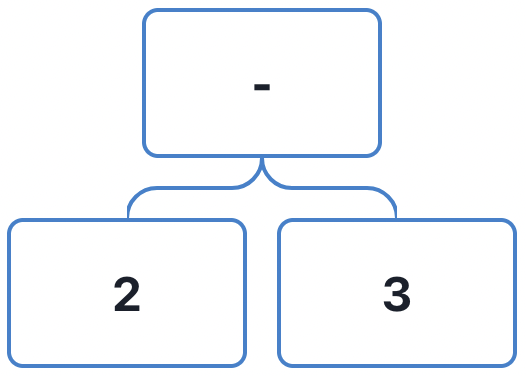
\includegraphics[scale=0.4]{trees/difference/beispiel_1_1.png}
      \caption{Baum von $2-3$.}
    \end{minipage}
    \begin{minipage}{.5\textwidth}
      \centering
      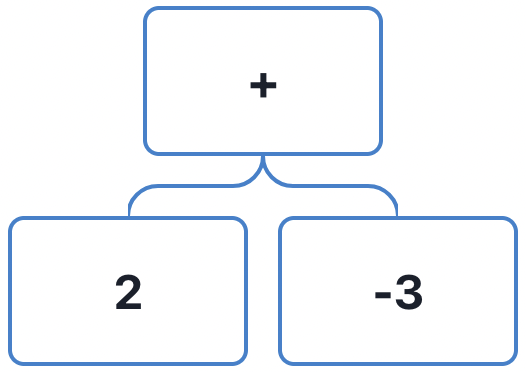
\includegraphics[scale=0.4]{trees/difference/beispiel_1_2.png}
      \caption{Anwedung der Differenzen-Transformation.}
    \end{minipage}
  \end{figure}
  \begin{figure}[h]
    \centering
    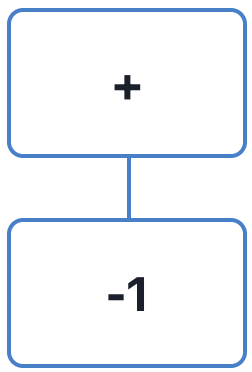
\includegraphics[scale=0.4]{trees/difference/beispiel_1_3.png}
    \caption{Die vollständig vereinfachte Summe.}
  \end{figure}
  In diesem Beispiel wird die Vereinfachung des Terms $2-3$ betrachtet. Dieser wird zuerst in eine Summe
  umgeschrieben und dann durch den Algorithmus zur Vereinfachung einer Summe zu $-1$ vereinfacht.
\end{example}

\subsubsection{Vereinfachung einer Division}
Sind Zähler und Nenner rationale Zahlen, wird die Division zu einem Bruch umgeschrieben.
Sonst wird die Quotienten-Transformation \lab{def:quotienten-transformation} angewandt.

\begin{example}
  \begin{figure}[h]
    \begin{minipage}{.5\textwidth}
      \centering
      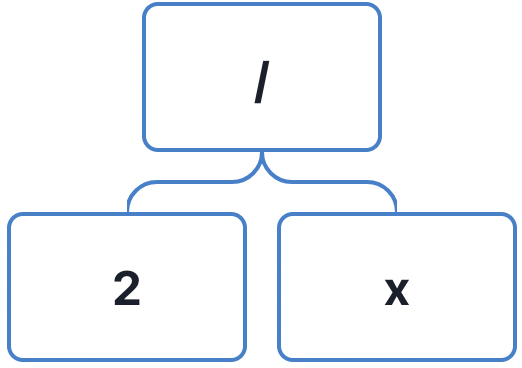
\includegraphics[scale=0.4]{trees/division/beispiel_1_1.png}
      \caption{Baum von $\frac{2}{3}$.}
    \end{minipage}
    \begin{minipage}{.5\textwidth}
      \centering
      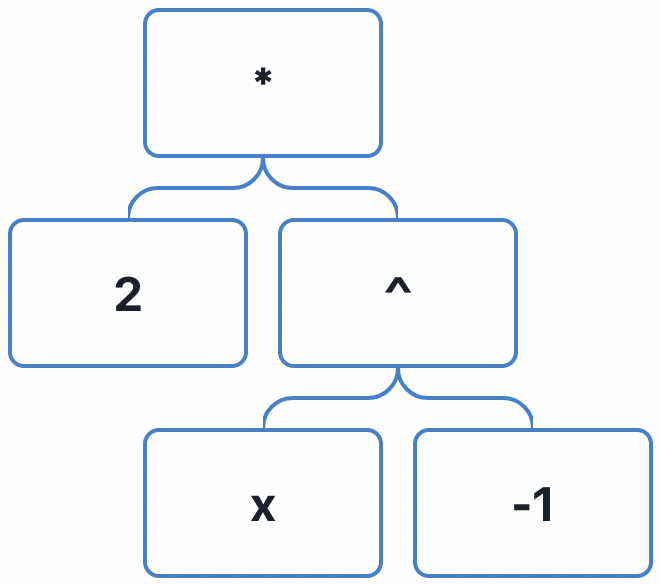
\includegraphics[scale=0.4]{trees/division/beispiel_1_2.png}
      \caption{Anwendung der Quotienten-Transformation.}
    \end{minipage}
  \end{figure}
  Der Term $\frac{2}{x}$ wird in ein Produkt umgeschrieben und dann so weit es geht vereinfacht. In diesem Fall
  ist der Term allerdings schon vollständig vereinfacht.
\end{example}

\subsubsection{Vereinfachung einer Potenz}
\begin{enumerate}
  \item Ist die Basis 0, wird die Identitäten-Transformation 4 \lab{def:identitaeten_transformation} angewandt.
  \item Ist der Exponent eine ganze Zahl:
        \begin{enumerate}
          \item Ist der Exponent 0 oder 1, wird die 6. beziehungsweise 7. Identitäten-Transformation
                \lab{def:identitaeten_transformation} angewandt.
          \item Ist die Basis eine rationale Nummer, so wird die 3. numerische Transformation
                \lab{def:numerische_transformation} und auf deren Ergebnis die numerische 
                Transformation 4 \lab{def:numerische_transformation} angewandt.
          \item Ist die Basis eine Potenz, wird die 2. Potenz-Transformation \lab{def:potenz_transformation} angewandt.
          \item Ist die Basis ein Produkt, wird die 3. Potenz-Transformation \lab{def:potenz_transformation} angewandt.
        \end{enumerate}
  \item Trifft keiner der oberen Fälle zu, wird nichts vereinfacht.
\end{enumerate}

\begin{example}
  \begin{figure}[h]
    \begin{minipage}{.5\textwidth}
      \centering
      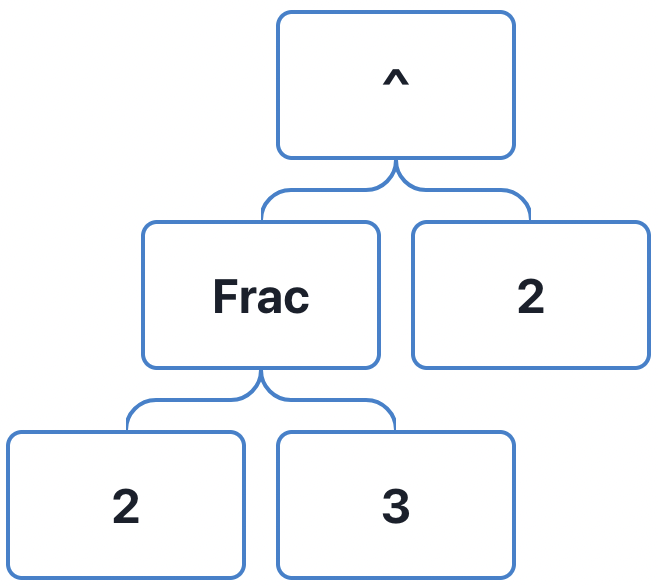
\includegraphics[scale=0.4]{trees/power/beispiel_1_1.png}
      \caption{Baum des Ausdruckes $\frac{2}{3}^2$.}
    \end{minipage}
    \begin{minipage}{.5\textwidth}
      \centering
      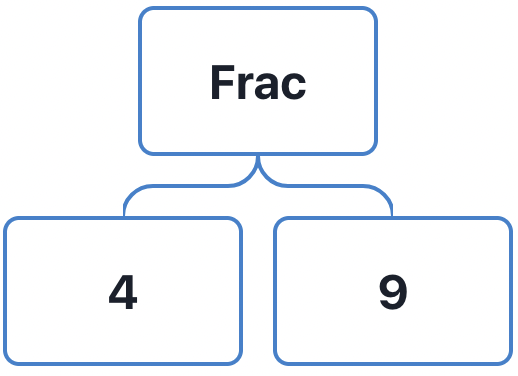
\includegraphics[scale=0.4]{trees/power/beispiel_1_2.png}
      \caption{Anwendung der 3. numerische Transformation.}
    \end{minipage}
  \end{figure}
  Da der Exponent im Term $\frac{2}{3}^2$ eine ganze Zahl ist, wird hier die 3. numerische Transformation angewandt. 
  Der resultierende Bruch wird nicht weiter durch die 4. numerische Transformation vereinfacht,
  da er schon vollständig vereinfacht ist.
\end{example}

\begin{example}
  \begin{figure}[h!]
    \begin{minipage}{.5\textwidth}
      \centering
      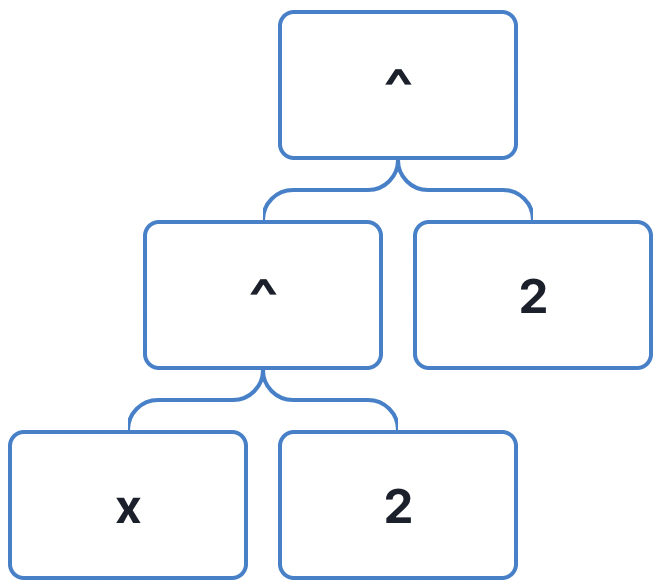
\includegraphics[scale=0.4]{trees/power/beispiel_2_1.png}
      \caption{Baum von ${x^2}^2$.}
    \end{minipage}
    \begin{minipage}{.5\textwidth}
      \centering
      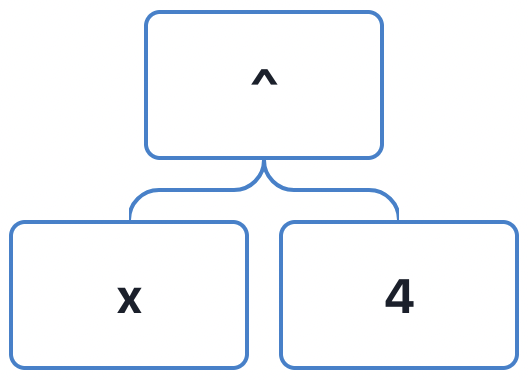
\includegraphics[scale=0.4]{trees/power/beispiel_2_2.png}
      \caption{Anwendung der 3. Potenz-Transformation.}
    \end{minipage}
  \end{figure}
  Der Term ${x^2}^2$ wird mithilfe der 3. Potenz-Transformation vereinfacht. 
\end{example}

\begin{example}
  \begin{figure}[h]
    \begin{minipage}{.5\textwidth}
      \centering
      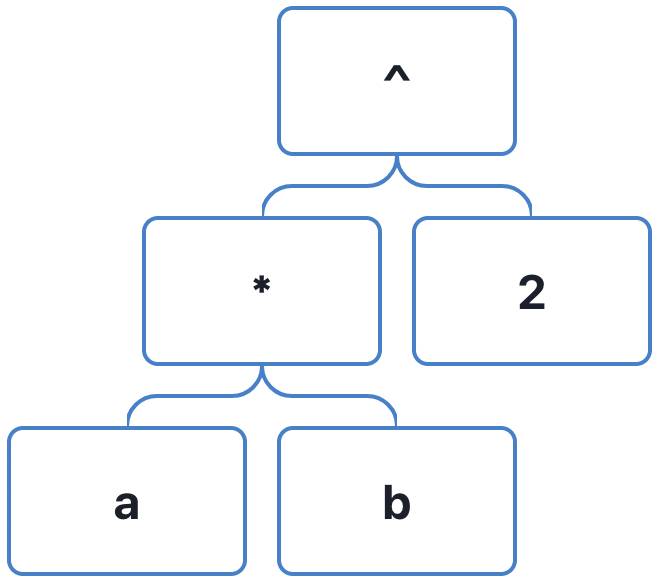
\includegraphics[scale=0.4]{trees/power/beispiel_3_1.png}
      \caption{Baum von ${(a*b)^2}$.}
    \end{minipage}
    \begin{minipage}{.5\textwidth}
      \centering
      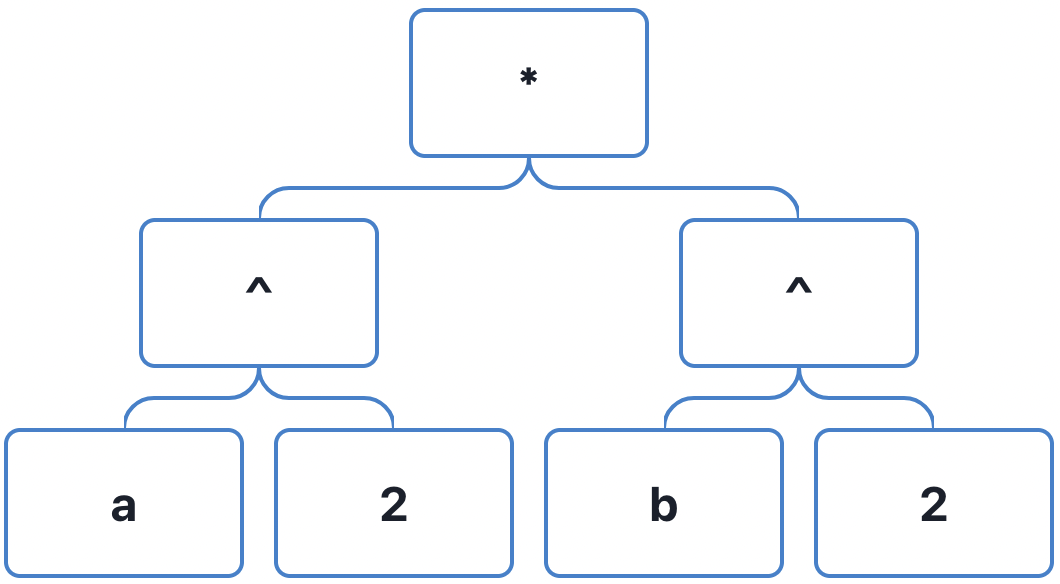
\includegraphics[scale=0.4]{trees/power/beispiel_3_2.png}
      \caption{Anwendung 2. Potenz-Transformation.}
    \end{minipage}
  \end{figure}
  Ist die Basis einer Potenz ein Produkt, wie etwa bei dem Term ${{(a*b)}^2}$, so wird die 2.
  Potenz-Transformation angewendet.
\end{example}

\subsubsection{Vereinfachung eines Produkts}
Ein Produkt wird vereinfacht, indem die folgenden 
Transformationen in genau dieser Reihenfolge angewendet werden.
\begin{enumerate}
  \item Assoziative Transformation \lab{def:assoziative_transformation}.
  \item Numerische Transformation 1 und 4 \lab{def:numerische_transformation}. 
        Im selben Schritt werden gleiche Terme miteinander multipliziert: Anwendung der Potenz-Transformation 1 
        \lab{def:potenz_transformation}, wenn beide Terme Potenzen mit gleicher Basis sind.
  \item Identitäten-Transformation 2 und 3 \lab{def:identitaeten_transformation}.
  \item Kommutative Transformation \lab{def:kommutative_transformation}.
\end{enumerate}

\begin{example}
  \begin{figure}[h]
    \begin{minipage}{.5\textwidth}
      \centering
      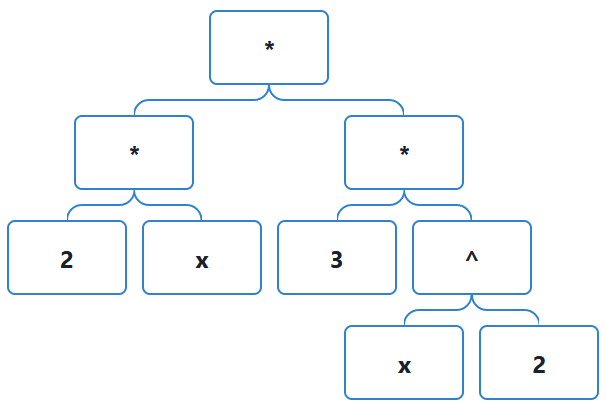
\includegraphics[scale=0.45]{trees/product/beispiel_1_1.png}
      \caption{Baum von $(2*x)*(3*x^2)$.}
    \end{minipage}
    \begin{minipage}{.5\textwidth}
      \centering
      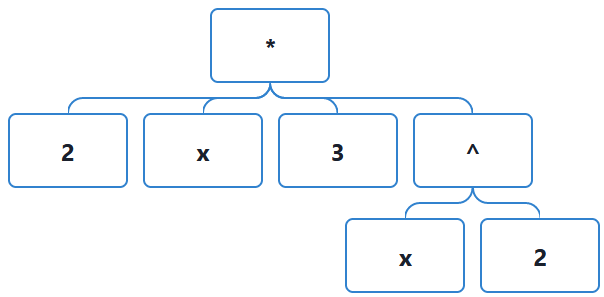
\includegraphics[scale=0.45]{trees/product/beispiel_1_2.png}
      \caption{Anwendung der assoziativen Transformation.}
    \end{minipage}
  \end{figure}
  \begin{figure}[h]
    \centering
    \includegraphics*[scale=0.5]{trees/product/beispiel_1_3.png}
    \caption{Anwendung der 1. numerischen Transformation und der 1. Potenz-Transformation}
  \end{figure}
  In diesem Beispiel wird der Term $(2*x)*(3*x^2)$ betrachtet. Zuerst wird die assoziative Transformation angewandt und
  die Operanden des Produkts werden mit den Operanden der Operanden ersetzt. Im nächsten Schritt wird die 1. numerische 
  Transformation sowie die 1. Potenz-Transformation angewendet, da die Terme $x$ und $x^2$ dieselbe Basis $x$ haben.
  Es wird keine Identitäten-Transformation angewandt, da weder $0$ noch $1$ Operanden des Produkts sind.
  Auch die kommutative Transformation verändert nichts an der Struktur des Terms, da alle Operanden schon in der richtigen
  Reihenfolge sind.
\end{example}

\subsubsection{Vereinfachung einer Summe}
Eine Summe wird vereinfacht, indem die folgenden 
Transformationen in genau dieser Reihenfolge angewendet werden.
\begin{enumerate}
  \item Assoziative Transformation \lab{def:assoziative_transformation}.
  \item Numerische Transformation 2 und 4 \lab{def:numerische_transformation}.
  \item Distributive Transformation \lab{def:distributive_transformation}.
  \item Identitäten-Transformation 1 und 3 \lab{def:identitaeten_transformation}.
  \item Kommutative-Transformation \lab{def:kommutative_transformation}.
\end{enumerate}

\begin{example}
  \begin{figure}[h]
    \begin{minipage}{.5\textwidth}
      \centering
      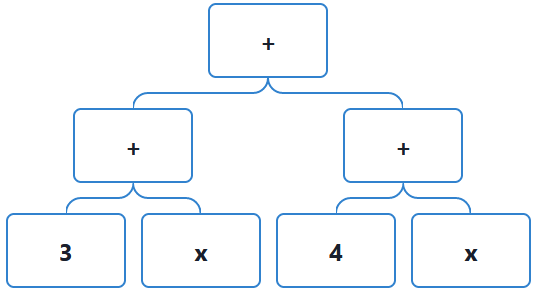
\includegraphics[scale=0.45]{trees/sum/beispiel_1_1.png}
      \caption{Baum von $(3+x)+(4+x)$}
    \end{minipage}
    \begin{minipage}{.5\textwidth}
      \centering
      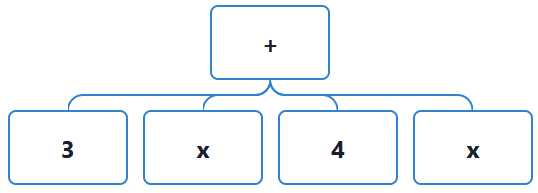
\includegraphics[scale=0.45]{trees/sum/beispiel_1_2.png}
      \caption{Anwendung der assoziativen Transformation.}
    \end{minipage}
  \end{figure}
  \begin{figure}[h]
    \begin{minipage}{.5\textwidth}
      \centering
      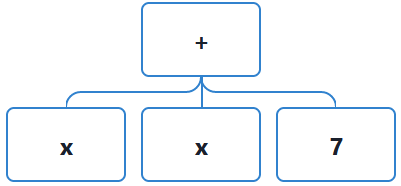
\includegraphics[scale=0.45]{trees/sum/beispiel_1_3.png}
      \caption{Anwendung der 2. numerischen Transformation.}
    \end{minipage}
    \begin{minipage}{.5\textwidth}
      \centering
      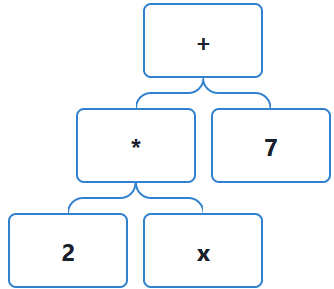
\includegraphics[scale=0.45]{trees/sum/beispiel_1_4.png}
      \caption{Anwendung der distributiven Transformation.}
    \end{minipage}
  \end{figure}
  \begin{figure}[h!]
    \centering
    \includegraphics*[scale=0.5]{trees/sum/beispiel_1_5.png}
    \caption{Anwendung der kommutativen Transformation.}
  \end{figure}
  In diesem Beispiel wird der Term $(3+x)+(4+x)$ betrachtet. Im 1. Schritt wird die assoziative Transformation angewandt.
  Darauf folgt die 2. numerische Transformation, bei der $4$ und $3$ zu $7$ zusammengefasst werden. 
  Im 3. Schritt wird $x+x$ im Zuge der distributiven Transformation zu $2*x$ vereinfacht.
  Es wird keine Identitäten-Transformation angewandt, da $0$ kein Operand der Summe ist.
  Durch die kommutative Transformation werden $7$ und $2*x$ miteinander vertauscht, da ganze Zahlen immer am 
  Anfang von Summen stehen müssen.
\end{example}

\subsubsection{Vereinfachung eines Ausdrucks}
Alle einzelnen Algorithmen werden in einem großen Vereinfachung Algorithmus kombiniert, 
der zuerst alle Operanden vereinfacht, und dann abhängig vom Typ des Ausdrucks die angemessene Vereinfachung vornimmt. \\
\newline
Ist der Ausdruck:
\begin{enumerate}
  \item Undefined → undefined.
  \item Ein Symbol oder eine ganze Zahl → Ausdruck wird nicht weiter vereinfacht.
  \item Ein Bruch → Der Bruch wird so weit gekürzt wie möglich.
  \item Eine Potenz → Vereinfachung einer Potenz.
  \item Eine Division → Vereinfachung einer Division.
  \item Ein Produkt → Vereinfachung eines Produkts.
  \item Eine Summe → Vereinfachung einer Summe.
  \item Eine Differenz → Vereinfachung einer Differenz
\end{enumerate}

Die Algorithmen, welche einen mathematischen Term vereinfachen können im Source Code unter
dem Pfad /server/cas/simplify oder online über \url{https://github.com/Flosi23/cas/tree/main/server/cas/simplify}
eingesehen werden.
Auch hier bietet sich zudem die Möglichkeit das Verhalten der Algorithmen auf der Website 
\url{https://cas.dotenv.de} selbst zu untersuchen. Der vereinfachte Baum ist nach Eingabe des
Ausdrucks unter dem Reiter \glqq Simplified Expression Tree\grqq{} zu finden.

\section{Schlusswort}

Modern Computeralgebrasysteme sind kein Hexenwerk. Komplizierte Operationen 
werden in immer kleinere Teilprobleme unterteilt bis das 
Problem für einen Computer einfach lösbar ist. So kann man die Vereinfachung eines
Ausdruckes unterteilen in die Vereinfachung einer Summe, Potenz, usw... Die Vereinfachung
einer Summe lässt sich nun auf die Anwendung verschiedener Transformationen reduzieren.\\

Was Computeralgebrasysteme aber so faszinierend macht, ist ihre Fülle an Funktionen und die Geschwindigkeit 
in der diese angewandt werden. In diesen beiden Punkten schneidet das im Zuge dieser Arbeit
geschriebene Programm schlecht ab. Da es weder eine eigene Programmiersprache noch vielfältige Algorithmen
zur Manipulation von Termen anbietet, kann es kaum als Computeralgebrasystem bezeichnet werden \lab{def:cas}.
Viel mehr sollte es als ein Hilfsmittel zur Visualisierung der automatischen Vereinfachung und des Parsing der 
Benutzereingaben angesehen werden. Das Ziel des Programms und dieser Arbeit wurde somit erreicht.

\section{Bibliografie}
\printbibliography[heading=none]
 
\end{document}